% TEX STUDIO MAGIC-COMMAND
% !TeX document-id = {21ffa6e2-6c8f-4532-897c-386dc477f19a}
% !TeX root = abstract.tex
% !TeX encoding = utf8
% !TeX TXS-program:compile = lualatex -file-line-error -synctex=1 -interaction=nonstopmode -halt-on-error %.tex
% !TeX TXS-program:quick = txs:///compile | txs:///view-pdf-internal --embedded

%-------------------------------------------------------------------------
% PD3予稿集テンプレート (main.tex)
% 作成: 金沢工大・情報工学科・鷹合研究室(2022,01/12)
%-------------------------------------------------------------------------

% テーマ番号
\def\THEMEID{2EP069}

% タイトル
\def\TITLEJP{観光案内アプリにおけるPWA活用に関する検討}
\def\TITLEEN{A Study on the Use of PWA in Tourist Information Apps}
% ここを書き換えて,表紙の「プロジェクトテーマ」という文字列がセル中心になるよう調整してください
\def\CENTERADJ{2.1} 

% 教員名
\def\PROFNAME{坂本 真仁 講師}

% アブストラクト(英文で書く)
% 最低:100ワード,最大:300ワード前後
% 英文部分については,句読点は半角にすること.つまり", "か". "を使う
\def\ABSTRACT{
It is difficult to achieve high usability because there are still people who cannot ensure sufficient communication environment depending on their region and income. Since there is a great demand for mobile devices, which are inexpensive electronic devices, it is important to improve the usability of mobile devices. Progressive Web Apps (PWA) are attracting attention as a means to achieve this. First, using a mobile-native tourist information application as a comparison target, we examined changes in usability when using a Web Standards API in a PWA. Next, we included PWA into a web app that maps tourist attractions and measured PWA performance using Lighthouse and network throttling. The results showed that many of the features implemented in mobile native tourist information apps can be implemented in PWA-based apps, and the cache management can reduce performance degradation. These results suggest that PWA can be used in tourist information apps to achieve high usability even in environments with communication infrastructure and financial constraints.
}

% キーワード(5個まで)
\def\KEYWORDS{PWA,Device Emulation,Real User Monitoring}

% 著者リスト
\def\AUTHORS{
\begin{minipage}{13.5cm}
4EP1-25~笹川 尋翔(SASAGAWA Hiroto)
\end{minipage}
}
\documentclass{tkglabs}
\begin{document}
\maketitle
\begin{multicols*}{2}

\section{はじめに}
\subsection{背景}
通信インフラへの投資が、モバイル通信システムの新しい世代の普及率に影響を及ぼしていることが指摘されている~\cite{Forge2020FormingA5GStrategyForDevelopingCountries}。通信インフラはモバイル通信サービスやオンラインサービスの基礎であるため、国々の間で激しい競争が行われているが、経済規模の違いから発展途上国や地方自治体は投資される側として不利である。

モバイル通信システムの世代が新しくなるにつれ、モバイル通信技術を導入するための費用が増加する傾向にある。例えば、モバイル通信システムの世代が新しいほど使用する周波数帯が高くなる傾向にあるが、これは1つの基地局が対応できる通信範囲が狭くなることを意味する。これにより、特定のカバレッジを確保する場合にかかる基地局などの設備費用が増加する。

モバイル端末は安価である一方で、利用時には移動体通信が行われるため通信環境が変化しやすく、一定のユーザビリティーを確保することが難しい。このような問題を解決するために提案されている技術がPWA (Progressive Web Apps)である。PWAはモバイルネイティブアプリに代表される、プラットフォーム固有のアプリのユーザビリティーを提供するWebの技術である。

位置情報は、地図、カーナビゲーション、マーケティング、タクシーの配車、ゲーム、家族や友人と位置情報を共有するアプリなどで活用されている。これらのサービスによって位置情報技術の認知度がより向上し、その認知度の高まりが位置情報市場の拡大を支えていると考えられる。屋外の位置情報に関連する市場の規模は、国内では2025年度までに約1,900億円に拡大すると予想されている~\cite{MIC2023InformationStatistics}。
\subsection{目的}
観光案内アプリにPWAを導入する際の課題を明らかにすることを目的として、1) 関連研究で行われていたアプリのパフォーマンスの評価方法の問題点を指摘し、アプリのパフォーマンスをより正確に計測するための方法を示す。2) 新たに提案したパフォーマンスの計測方法を用いて、Service Workerのキャッシュ戦略を活用した場合の観光案内アプリのパフォーマンスを算出し、それぞれのキャッシュ戦略がどの程度効果的であるのかを示す。3) 新たに提案した方法でパフォーマンスを評価した場合に生じる問題点を指摘し、どのような改善が求められるのかを示す。
\section{関連研究}
Redditから画像とテキストを取得して表示する機能を、PWAとAndroidのネイティブアプリに実装し、アプリの最初のアクティビティが起動するまでの時間や、アプリのアイコンをタップしてからツールバーがレンダリングされるまでの時間を計測した研究がある~\cite{Andreas2018ProgressiveWebApps}。レンダリング時間が高速であり、プラットフォームに準拠したAPIを使用しており、専有する容量が小さいというPWAの特徴を根拠として、クロスプラットフォーム分野での競争力が高いと結論付けている。

現在のクロスプラットフォームフレームワークはプラットフォーム間で技術を統一できない~\cite{Majchrzak2018ProgressiveWebApps}。関連研究では、この問題を解決するための方法の1つとしてPWAを挙げている。PWAは単一のコードで複数のプラットフォームに対応できる点で他のクロスプラットフォームフレームワークとは異なる。PWAのようなクロスプラットフォームフレームワークの登場により学習工数やコストが削減され、市場投入までの時間が短縮される。
\section{研究内容}
観光案内アプリはユーザーが受け取るコンテンツが多いという特徴があるため、パフォーマンスが低下しやすい。PWAの構成要素のうち、Service Workerはパフォーマンスの低下を防ぐのに有用であるとされている。そのため、Service Workerを使用した際の観光案内アプリのパフォーマンスを評価する。

Webアプリの品質測定ツールであるLighthouseを用いて、モバイル端末の幅、高さ、性能をエミュレートしながらパフォーマンスを計測する。パフォーマンスを計測する際は、これらのエミュレーションに加えて、ネットワークスロットリングを使用したモバイル端末の通信環境のエミュレーションを行う。なぜなら、4G以前のモバイル通信システムはIEEE 802.11acなどの広く普及している無線LANの標準規格に比べて帯域幅が狭いため、無線LANに接続した端末でネットワークエミュレーションを行わずにパフォーマンスを計測すると、実際のモバイル端末でのパフォーマンスを正確に計測できない可能性が高いためである。ネットワークスロットリングとはインターネットの速度を意図的に低下させ、低帯域の状態をエミュレートすることである。この研究では、より正確なデータを得るために、パケットレベルのスロットリングを使用してパフォーマンスを計測する。パケットレベルのスロットリングを行うためにThrottleというライブラリを使用する。

\section{評価}
Lighthouseとネットワークスロットリングを使用して、それぞれの都道府県の観光地図を読み込んだ際のパフォーマンスを計測した。キャッシュ戦略ごとのパフォーマンス指標の値の平均を図~\ref{figure:Service Workerを使用しなかった場合のパフォーマンス}、~\ref{figure:画像をキャッシュした場合のパフォーマンス}、~\ref{figure:Same-Originのネットワークレスポンスをキャッシュした場合のパフォーマンス}に示す。
\begin{figure}
  \centering
  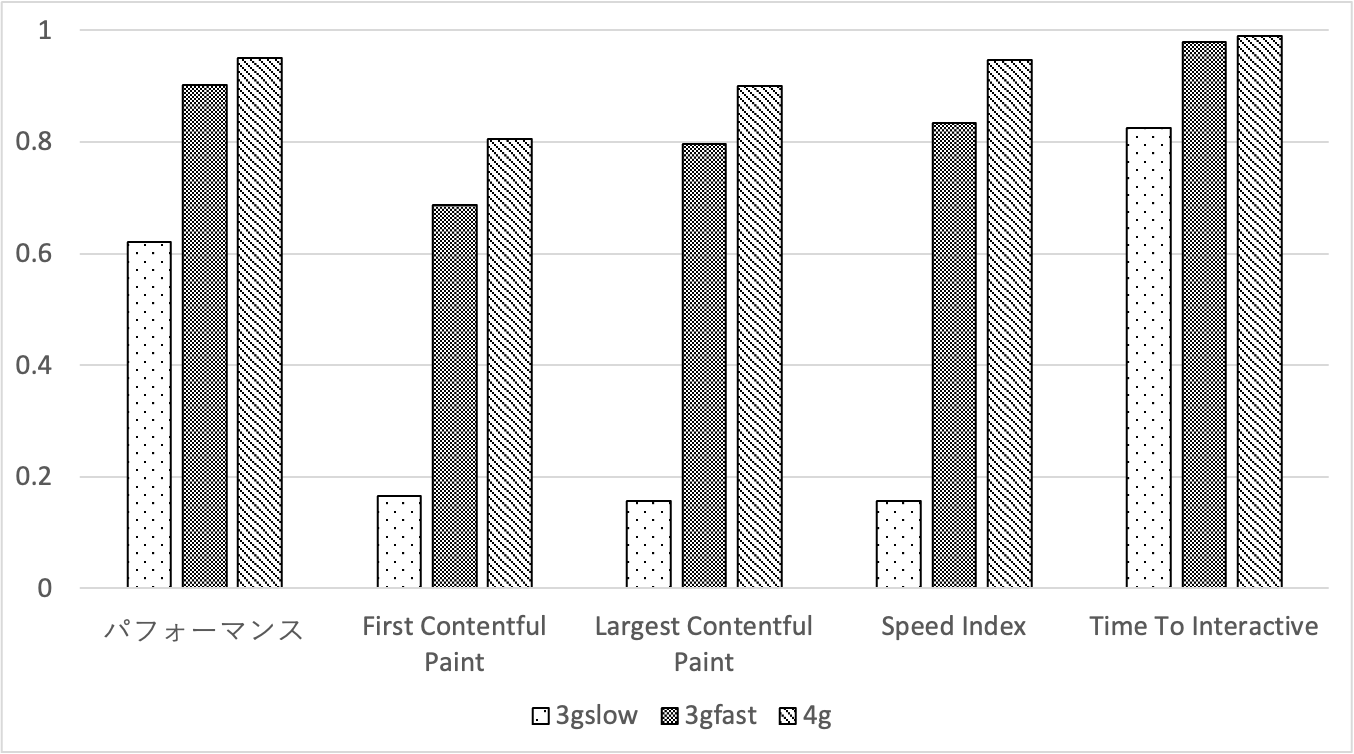
\includegraphics[width=\textwidth]{images/without_service_worker.png}
  \figcap{Service Workerを使用しなかった場合のパフォーマンス}{Performance without Service Worker}{figure:Service Workerを使用しなかった場合のパフォーマンス}
\end{figure}
\begin{figure}
  \centering
  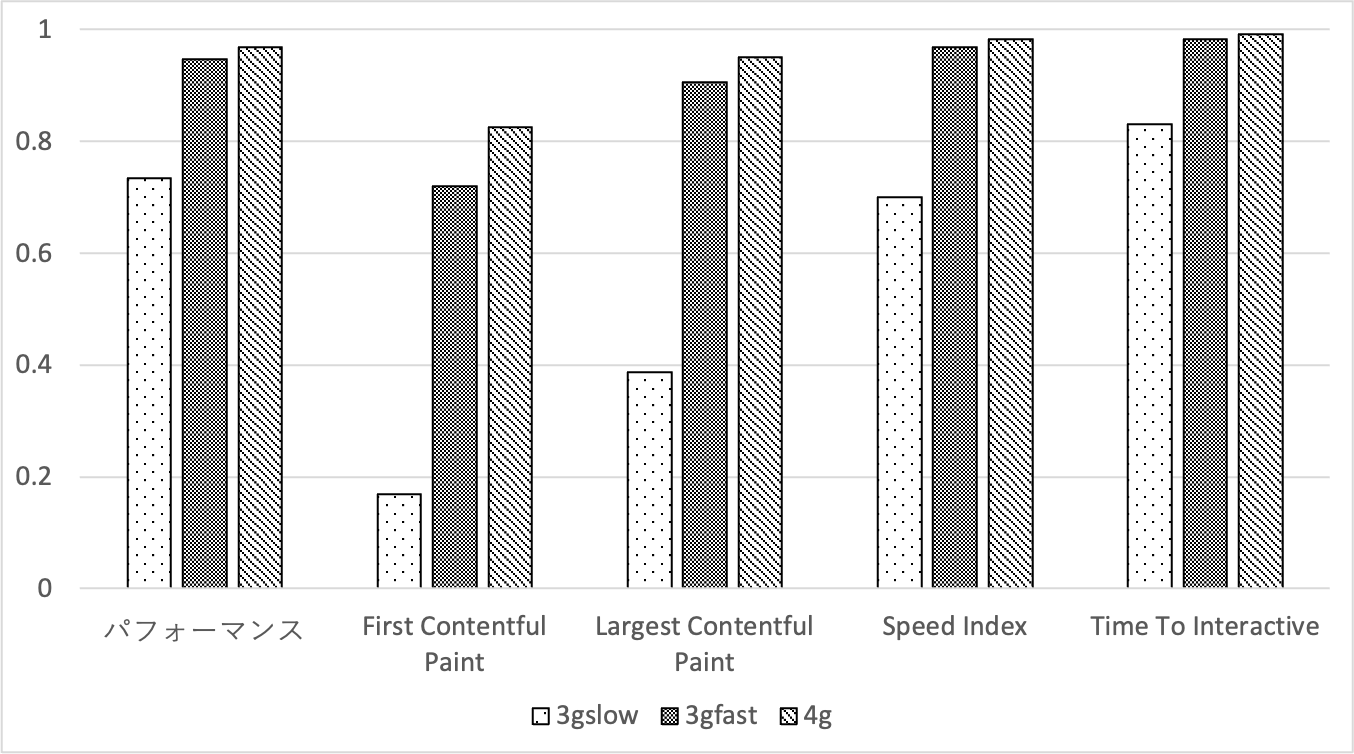
\includegraphics[width=\textwidth]{images/service_worker_cache_images.png}
  \figcap{画像をキャッシュした場合のパフォーマンス}{Performance when caching images}{figure:画像をキャッシュした場合のパフォーマンス}
\end{figure}
\begin{figure}
  \centering
  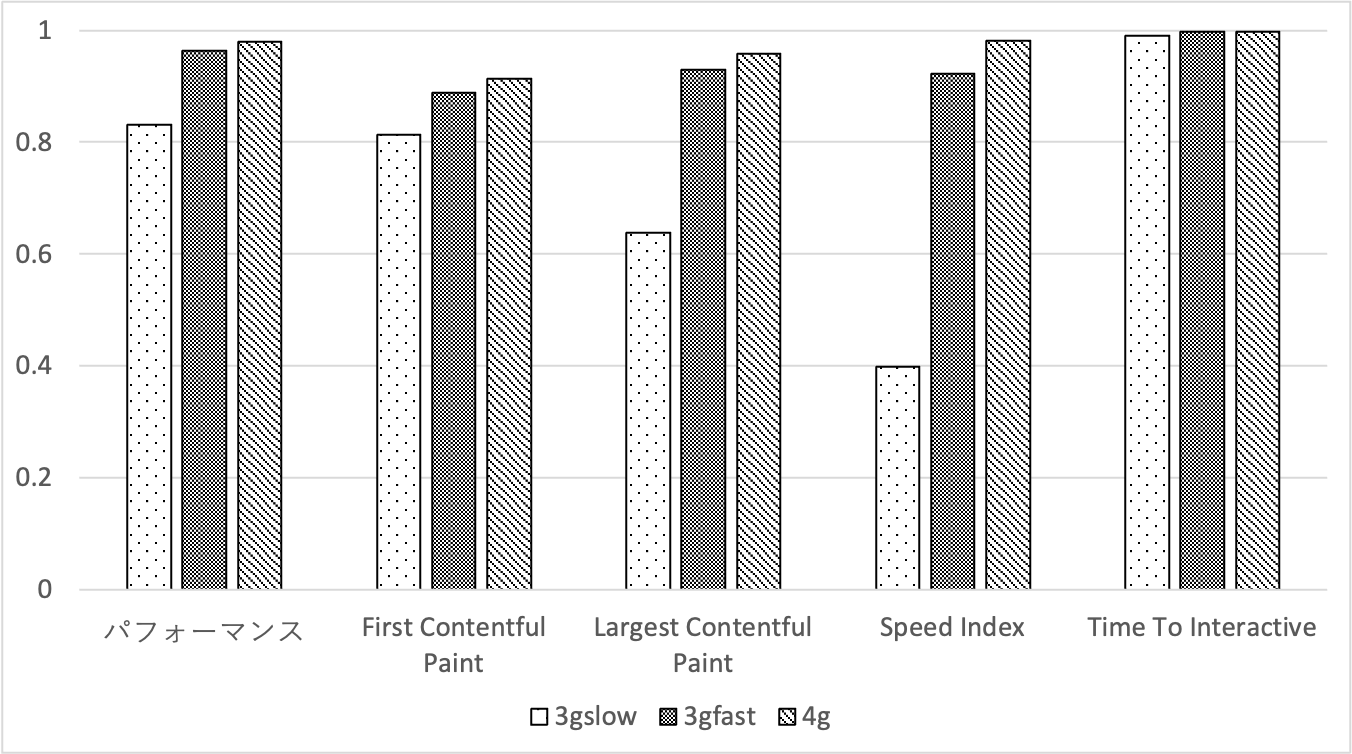
\includegraphics[width=\textwidth]{images/service_worker_cache_same_origin.png}
  \figcap{Same-Originのネットワークレスポンスをキャッシュした場合のパフォーマンス}
  {Performance when caching Same-Origin network responses}{figure:Same-Originのネットワークレスポンスをキャッシュした場合のパフォーマンス}
\end{figure}
画像をキャッシュした場合はFCP (First Contentful Paint)が最も通信速度の低下の影響を受けやすく、SI (Speed Index)が最もその影響を受けにくいことが分かる。逆に、Same-Originのネットワークレスポンスのキャッシュした場合はSIが最も通信速度の低下の影響を受けやすく、FCPが最もその影響を受けにくいことが示されている。

Same-Originのネットワークレスポンスをキャッシュした場合はいずれのネットワーク環境においてもTTI (Time To Interactive)がほぼ1である。対照的に、画像をキャッシュした場合のTTIはService Workerを使用しなかった場合のTTIとほとんど同じであるため、画像のキャッシュはTTIにほとんど影響を及ぼさないことが分かる。

\section{まとめ}
\subsection{考察}
Same-Originのネットワークレスポンスをキャッシュした場合はSIの値が小さく、画像をキャッシュした場合はFCPの値が小さい。Same-Originのネットワークレスポンスはいずれも画像に比べてファイルサイズが小さいため、Same-Originのネットワークレスポンスをキャッシュした場合はSIの値が小さくなりやすいと考えられる。一方で画像をキャッシュした場合は、ページの最初のコンテンツをレンダリングするために必要なHTMLをサーバーから取得する必要があるため、FCPが小さくなりやすいと考えられる。TTIについては、JavaScriptのイベントハンドラーの実行が悪影響を及ぼしていると考えられる。特に、Webアプリに観光地図を実装する場合は、サムネイル表示や詳細表示を実現するために、mouseoverイベントやclickイベントを、観光名所を表すノード単位で監視するため、イベントハンドラーの実行時間が長くなりやすい。PWAの導入後のパフォーマンスを計測する方法は改善の余地がある。例えば、ユーザーのインタラクションの遅延を計測することで、実際のユーザビリティーをより正確に評価できる。

\subsection{結論}
LighouseとThrottleを使用してパフォーマンスを計測した場合は、PWAのインタラクティブ性を評価できないことが明らかになった。PWAのインタラクティブ性を評価できる可能性がある方法としては、Interaction to Next Paintを使用したユーザーのアクションに対する応答速度の計測や、Long Tasks APIを使用したLong Tasksの検出とその実行時間の計測がある。これらの方法は現在レビュー段階にあるため、さらなる検証が必要である。これらの方法によって算出される指標の値がPWAのインタラクティブ性とどの程度関連しているのかを明らかにすることで、PWAのパフォーマンスをより正確に算出できるようになり、PWAの活用が促進されると考えられる。

\begin{thebibliography}{9}
\bibitem{Forge2020FormingA5GStrategyForDevelopingCountries} S.Forge and K.Vu.Forming a 5g strategy for developing countries: A note for policy makers.\textit{Telecommunications Policy},Vol,44,No.7,2020.
\bibitem{MIC2023InformationStatistics} 総務省.情報通信白書令和5年版.\url{https://www.soumu.go.jp/johotsusintokei/whitepaper/r05.html}
\bibitem{Andreas2018ProgressiveWebApps} A.Biørn-Hansen,et al.Progressive web apps for the unified development of mobile applications.In \textit{Web Information Systems and Technologies},pp.64–86,Cham,2018.Springer International Publishing
\bibitem{Majchrzak2018ProgressiveWebApps} T.A.Majchrzak,et al.Progressive web apps: the definite approach to cross-platform development? In \textit{Hawaii International Conference on System Sciences},pp.5735–5744.IEEE Computer Society,January 2018.
\end{thebibliography}
\end{multicols*} 
\end{document}